%%%%%%%%%%%%%%%%%%%%%%%%%%%%%%%%%%%%%%%%%
% University/School Laboratory Report
% LaTeX Template
% Version 3.0 (4/2/13)
%
% This template has been downloaded from:
% http://www.LaTeXTemplates.com
%
% Original author:
% Linux and Unix Users Group at Virginia Tech Wiki
% (https://vtluug.org/wiki/Example_LaTeX_chem_lab_report)
%
% License:
% CC BY-NC-SA 3.0 (http://creativecommons.org/licenses/by-nc-sa/3.0/)
%
%%%%%%%%%%%%%%%%%%%%%%%%%%%%%%%%%%%%%%%%%

%----------------------------------------------------------------------------------------
%	PACKAGES AND DOCUMENT CONFIGURATIONS
%----------------------------------------------------------------------------------------

\documentclass[twocolumn]{article}

\usepackage{mhchem} % Package for chemical equation typesetting
\usepackage{siunitx} % Provides the \SI{}{} command for typesetting SI units
\usepackage{hyperref}
\usepackage{graphicx} % Required for the inclusion of images
\usepackage{tabularx}
\usepackage{float}
\usepackage{algorithm}
\usepackage{algpseudocode}
\usepackage{bm}
\usepackage{multirow}% http://ctan.org/pkg/multirow
\usepackage{hhline}% http://ctan.org/pkg/hhline


\setlength\parindent{0pt} % Removes all indentation from paragraphs

\renewcommand{\labelenumi}{\alph{enumi}.} % Make numbering in the enumerate environment by letter rather than number (e.g. section 6)

%\usepackage{times} % Uncomment to use the Times New Roman font

%----------------------------------------------------------------------------------------
%	DOCUMENT INFORMATION
%----------------------------------------------------------------------------------------

\title{UC Davis STA 242 2015 Spring Assignment 2} % Title
\author{Wenhao \textsc{Wu}, 9987583} % Author name
\date{\today} % Date for the report

\begin{document}
\maketitle % Insert the title, author and date

% If you wish to include an abstract, uncomment the lines below

\section{Data Structure and Algorithm Design}
A \texttt{BMLGrid} instance contains 3 components:
\begin{description}
    \item[\texttt{grid}] A \texttt{r}-by-\texttt{c} integer matrix. If
    \texttt{grid[i,j]==0}, then there is no car on the crossing of $i$-th row
    and $j$-th column; if \texttt{grid[i,j]==1}, there is a red car on that
    grid; if \texttt{grid[i,j]==2}, there is a blue car on that. In our program,
    when \texttt{grid} is indexed, it is treated as a vector (1-D).
    \item[\texttt{blue}] An integer vector contains the 1-D indices of
    all blue cars in \texttt{grid}.
    \item[\texttt{red}] An integer vector contains the 1-D indices of
    all red cars in \texttt{grid}.
\end{description}
We define 2 key functions that returns a vector of 1-D
indices in \texttt{grid}
\begin{description}
    \item[\texttt{idx\_right()}] Given an input vector of 1-D indices in
    \texttt{grid}, return a vector of 1-D indices in \texttt{grid} for grids to
    the \emph{right} of the input grids.
    \item[\texttt{idx\_up()}] Given an input vector of 1-D indices in
    \texttt{grid}, return a vector of 1-D indices in \texttt{grid} for grids to
    the \emph{up} of the input grids.
\end{description}
Upon each step, we use \texttt{idx\_up()}(\texttt{idx\_right()}) to check in
\texttt{grid} whether the grids to the up(right) of the grids represented by
\texttt{blue}(\texttt{red}) is occupied, then update the cars' indices
\texttt{blue}(\texttt{red}) and the grid state \texttt{grid} accordingly.

The R script file to test the basic design of our code is \textbf{Test.R}.

\section{Verifying and Profiling}
In order to verify the functionality of our BML simulation, we use package
`animation' to generate a short movie showing how cars move on the grid. This
function has also been incorporated in our final BMLGrid package.

We have also improved the performance of our code using Rprof(), which
originally happens at commit e8fcb63. We demonstrate this process by recreating
the code for the original algorithm in \textbf{TestProfiling\_original.R} and
compare it with our improved code which is profiled in \textbf{TestProfiling.R}. Again
we take the total running time over 10 repetitions of constructing a BMLGrid
object with $r=100$, $c=99$, $\rho=0.3$ and the same number of red and blue
cars, then run the BML simulation for 10000 steps. The generated profiling files
for the original and the modified code are \textbf{ProfBMLGridOriginal.out} and
\textbf{ProfBMLGrid.out}, respectively. When examining the profiling result for
the original code, the first few lines are shown in Table~\ref{tab:profile_original}. We
notice that function \texttt{ifelse()} has a very high overhead, and confirm
this observation by using \texttt{lines=``show''} option in
\texttt{summaryRprof()} function, which shows that \texttt{ifelse()} in line 68
and 78 have a self.time of 7.82 and 5.96, respectively. The total sampling.time
is 31.98.

\begin{table}[!t]
    \renewcommand{\arraystretch}{1.3}
    \caption{Rpof summary for the original code (by.self).}
    \label{tab:profile_original}
    \centering
    \begin{tabular}{c|cccc}
        \hline
         & self.time & self.pct & total.time & total.pct \\
        \hline
        ``ifelse'' & 13.46 & 42.09 & 13.74 & 42.96 \\
        ``eval'' & 8.82 & 27.58 & 31.98 & 100.00 \\
        ``\%\%'' & 2.88 & 9.01 & 2.88 & 9.01 \\
        \ldots & \ldots & \ldots & \ldots & \ldots \\
        \hline
    \end{tabular}
\end{table}

To reduce this overhead, we notice that in our design the order of \texttt{red}
and \texttt{blue} vector component of a \texttt{BMLGrid} instance does not
matter at all. Consequently, a more effective method to update these two components is to
simply concatenate a sub-vector of indices of the cars moved and a
sub-vector of indices of the cars unmoved. As a result, our modified code has
reduced the sampling.time to 20.9, a good 1/3 of improvement in running speed.

\section{Simulation Results}
\subsection{Behavior of the BML model}
We pick a $r=100$, $c=99$ grid in which the number of blue cars and red cars
are the same. After $N = 10000$ steps, we observe a phase transition in the
final state of the grid at $\rho\approx 0.38$. The final states of the grid for
$\rho = 0.2, 0.33, 0.38, 0.43, 0.5$ are plotted in Fig.~\ref{fig:final_state}.
When $\rho$ is small, the grid eventually enters an ordered state where the red
and blue cars form a few sparse top-left-to-bottom-right diagonal strips that
moves right/upward with little interference. When $\rho$ is large, the grid eventually
enters a stale state where the red and blue cars form a few dense
top-right-to-bottom-left diagonal strips that stopped moving any more. At
$\rho\approx 0.38$, we observed a state transition where after $N = 10000$
steps, the grid is neither in a fully ordered, interference-free mode nor in a
complete grid lock.

\begin{figure}[!t]
    \begin{minipage}[b]{0.49\linewidth}
      \centering
      \centerline{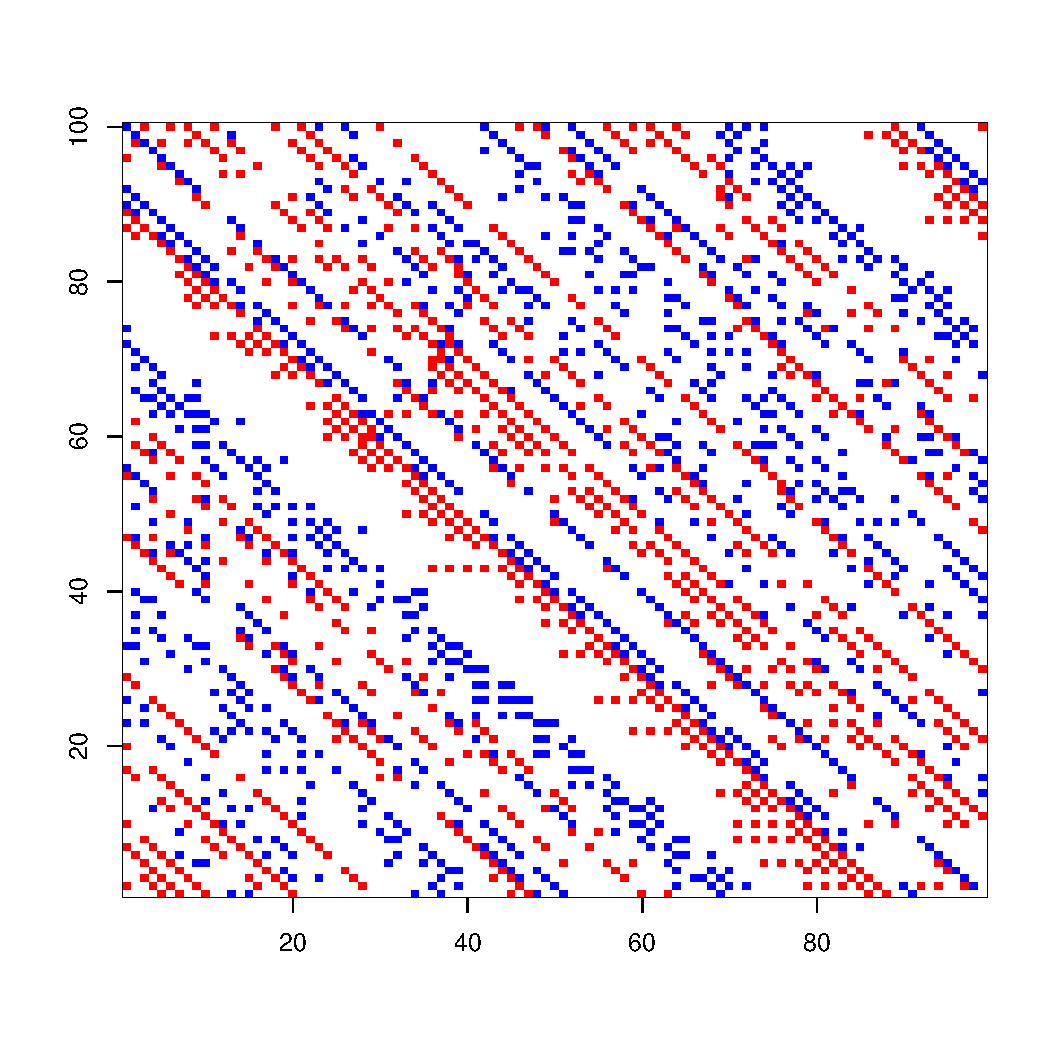
\includegraphics[width=4.0cm]{./figs/TestBehavior_100_99_10000_02_end.pdf}}
      \centerline{(a) $\rho = 0.2$}\medskip
    \end{minipage}
    \hfill
    \begin{minipage}[b]{0.49\linewidth}
      \centering
      \centerline{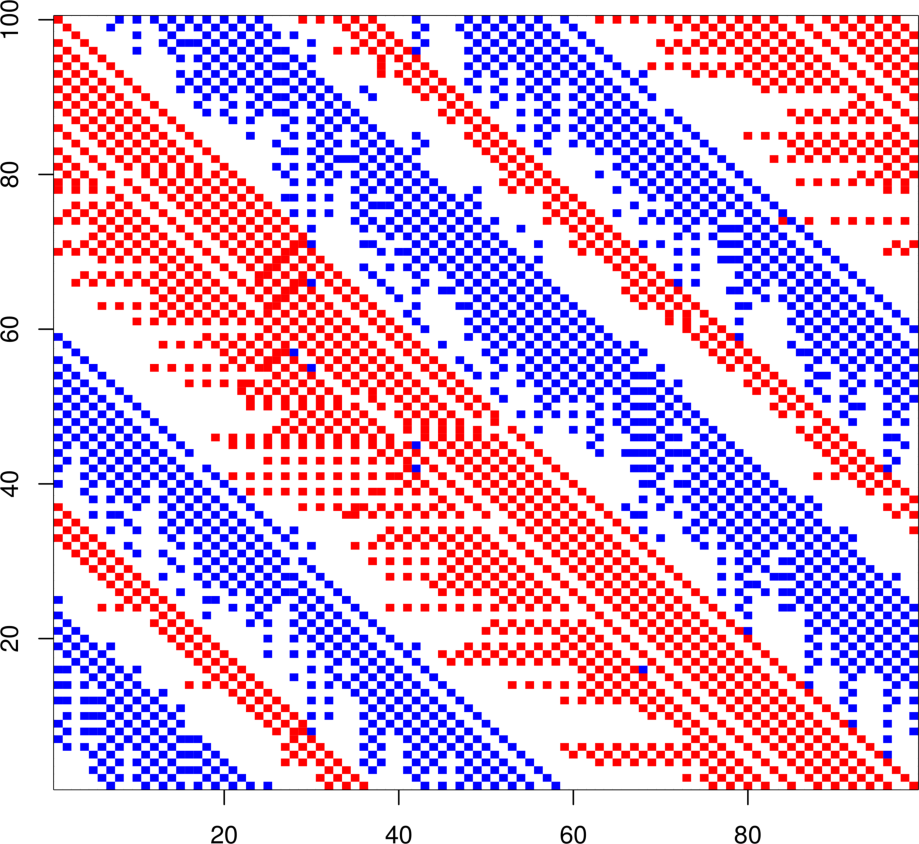
\includegraphics[width=4.0cm]{./figs/TestBehavior_100_99_10000_033_end}}
      \centerline{(b) $\rho = 0.33$}\medskip
    \end{minipage}
    \hfill
    \begin{minipage}[b]{0.49\linewidth}
      \centering
      \centerline{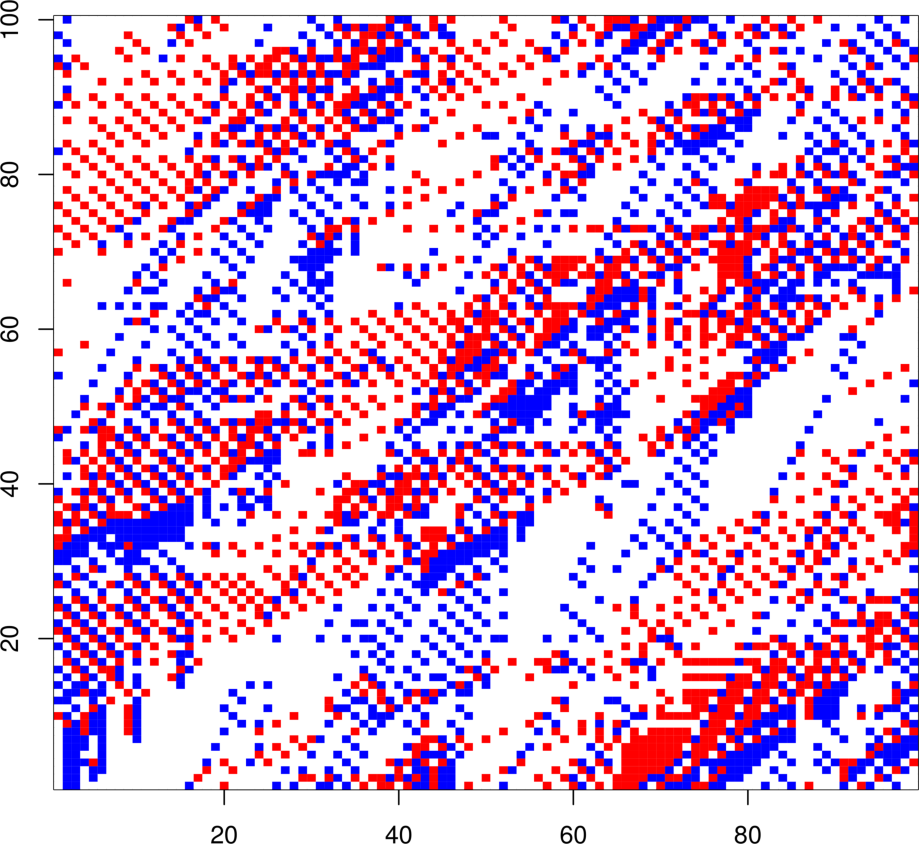
\includegraphics[width=4.0cm]{./figs/TestBehavior_100_99_10000_038_end}}
      \centerline{(c) $\rho = 0.38$}\medskip
    \end{minipage}
    \hfill
    \begin{minipage}[b]{0.49\linewidth}
      \centering
      \centerline{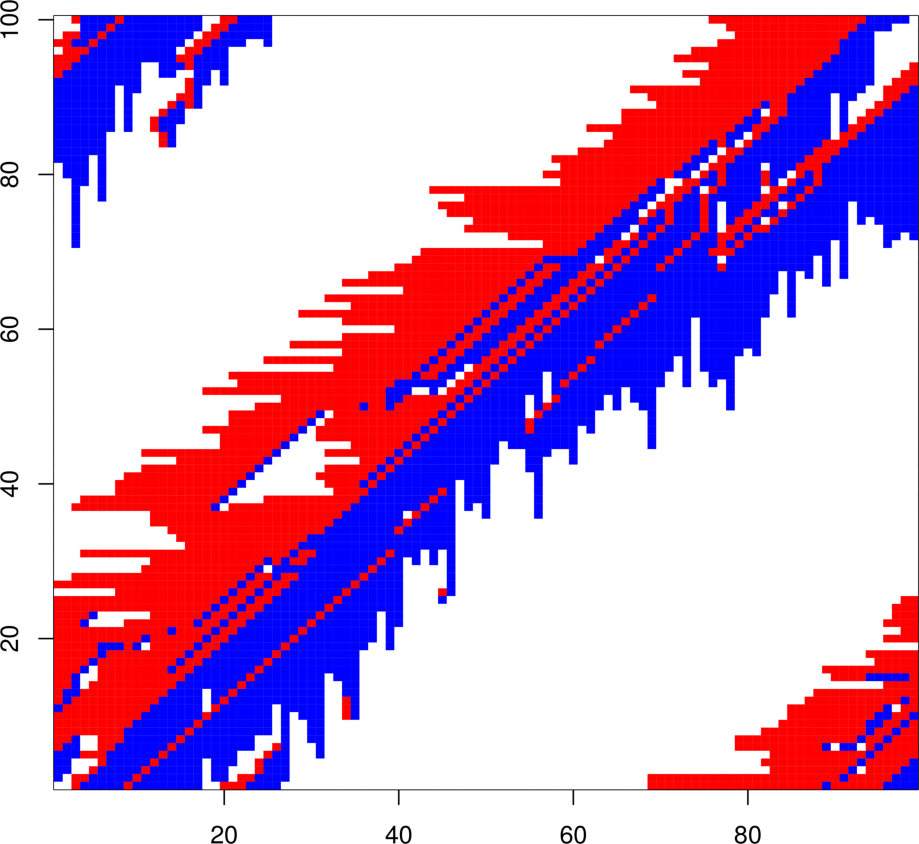
\includegraphics[width=4.0cm]{./figs/TestBehavior_100_99_10000_043_end}}
      \centerline{(d) $\rho = 0.43$}\medskip
    \end{minipage}
    \hfill
    \begin{minipage}[b]{1\linewidth}
      \centering
      \centerline{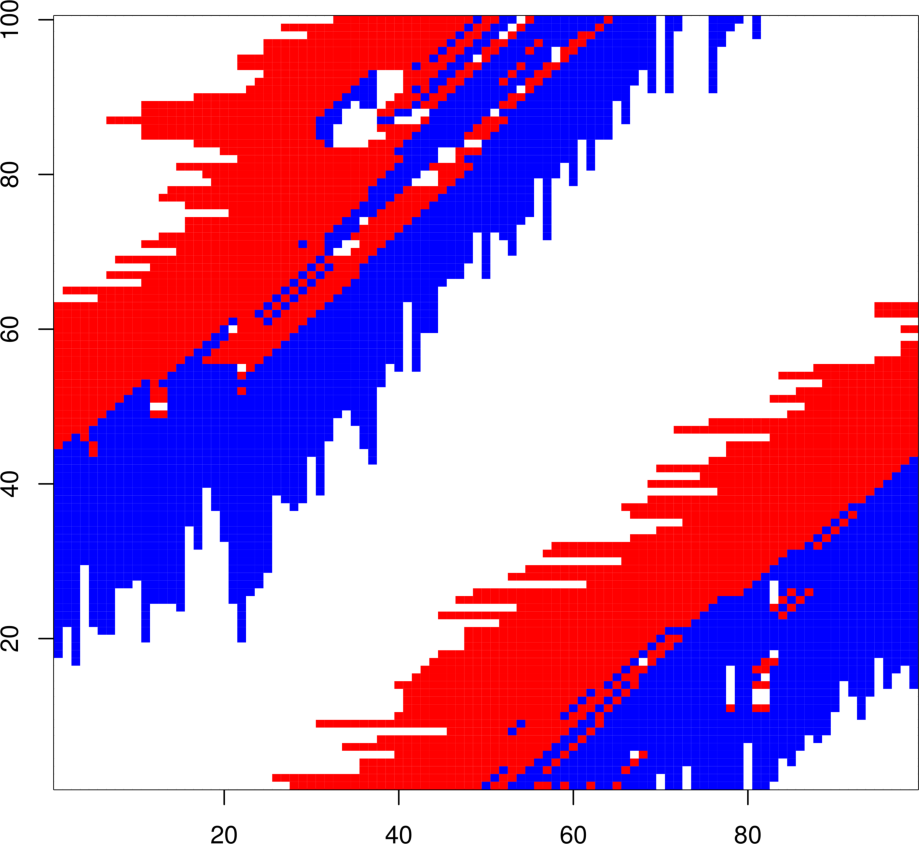
\includegraphics[width=4.0cm]{./figs/TestBehavior_100_99_10000_05_end}}
      \centerline{(e) $\rho = 0.5$}\medskip
    \end{minipage}
    \caption{Final state of a $100\times99$ grid with equal number of blue and
    red cars after 10000 steps for different car density $\rho$.}
    \label{fig:final_state}
\end{figure}

We further justify this phase transition by looking at the evolution of the
grid. In Fig.~\ref{fig:average_velocity}, we demonstrate how the average
velocity of blue cars change over time for different $\rho$. As we can see, when
$\rho$ is below a threshold, the smaller $\rho$ is, the quicker the average
speed reaches 1, indicating that their is no blockage for blue cars in the grid.
When $\rho$ is above a threshold, the larger $\rho$ is, the quicker the average
speed drops to 0, indicating there is a total grid lock. When $\rho\approx
0.38$, the average speed varies drastically and takes very long (or maybe
infinite) time to reach either the ordered state or the grid lock state. In
summary, the BML traffic model demonstrate a \emph{chaotic} behavior: the system
is mostly determinstic (except for the grid initialization), however a minor
change in parameter $\rho$ will result in a completely different future.

\begin{figure}[h]
    \centering
    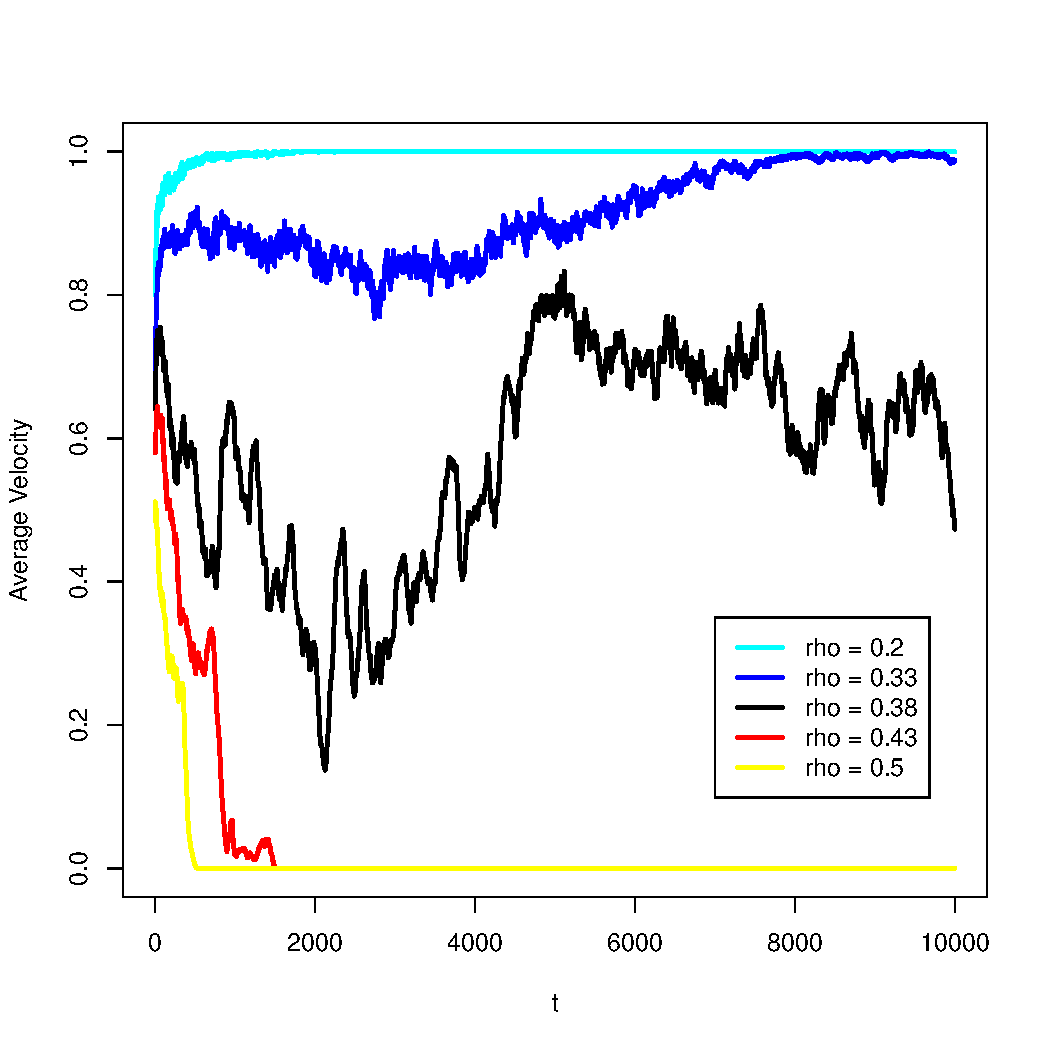
\includegraphics[width=2.5in]{figs/TestVelocity.pdf}
    \caption{The evolution of average velocity of the blue cars.}
    \label{fig:average_velocity}
\end{figure}

The R script file to demonstrate the behavior of BML model and measure the
average velocity are \textbf{TestBehavior.R} and
\textbf{TestAverageVelocity.R}, respectively.

\subsection{Code Performance}
In order to demonstrate the performance of our code, we measure the running time
of a function in which
\begin{itemize}
    \item A BMLGrid instance \texttt{g} with $r=c=128,256,512,1024$ and
    $\rho=0.1,0.2,9.3,0.4,0.5,0.6,0.7$ is contructed.
    \item A BML simulation for $N=10000$ steps is performed on \texttt{g}.
\end{itemize}
For each of the $4\times7 = 28$ instances, the running time is measured by
taking the average of 5 runs. We run this test on a Dell Precision T1700
workstation equipped with 16GB RAM and a Core i7-4790K CPU in Ubuntu 14.04 OS.
The result is plotted in Fig~\ref{fig:running_time}. When $\rho$ is smaller than
the threshold, the larger $\rho$ is, the longer the running time is. This is due
to the fact that the vector indexing/updating has complexity proportional to the
number of cars. When $\rho$ is greater than the threshold, the running time
dereases dramatically, thanks to our codes' capability to detect a grid lock
state and break from the iteration. As expected, the running time reaches its
peak when $\rho\approx0.38$. Also it is intuitively correct that the running
time is about proportional to the size of the grid (i.e. the square of the edge
length).

The R script file to test the running time of our BMLGrid key functions is
\textbf{TestRunningTime.R}.

\begin{figure}[h]
    \centering
    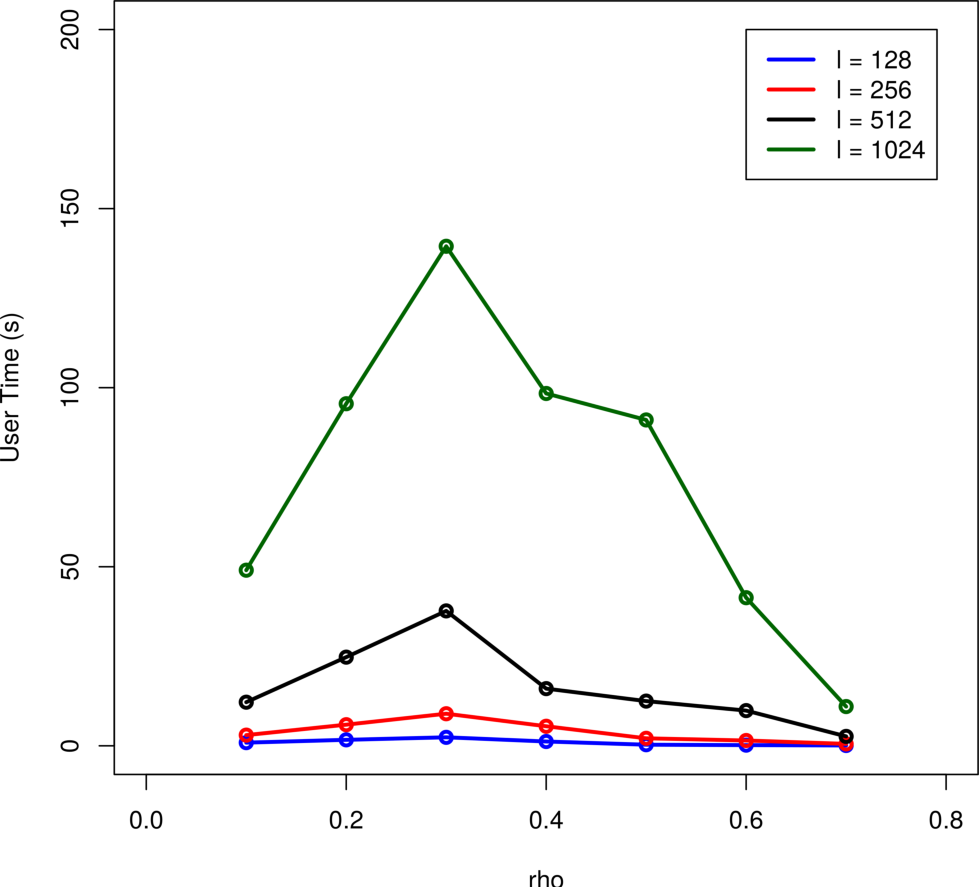
\includegraphics[width=2.5in]{figs/TestRunningTime.pdf}
    \caption{Average user time of a barebone BMLGrid simulation over 5
    repetitions for $\rho=0.1,0.2,9.3,0.4,0.5,0.6,0.7$ and
    $r=c=128,256,512,1024$.}
    \label{fig:running_time}
\end{figure}


\section{Build BMLGrid Package}
The BMLGrid package is developed in RStudio. We manually edit the
DESCRIPTION file and the package level object documentation file
BMLGrid-package.Rd, while NAMESPACE and other function
documentation files are generated with roxygen2. The source package is located
in directory \textbf{BMLGrid/}.

%\pagebreak
%	BIBLIOGRAPHY
%----------------------------------------------------------------------------------------

%\bibliographystyle{unsrt}
%\bibliography{myrefs}

%----------------------------------------------------------------------------------------


\end{document}